\documentclass[UTF8,zihao=-4]{ctexart}

\usepackage[a4paper,margin=1.8cm]{geometry}
\usepackage{amsmath,amssymb}
\usepackage{array,tabularx,longtable,multirow}
\usepackage{enumitem}
\usepackage{listings}
\usepackage{fancyhdr}
\usepackage{lastpage}
\usepackage{forest}
\usetikzlibrary{automata,positioning,arrows.meta}

\setCJKmainfont{Source Han Serif CN}
\setCJKsansfont{Source Han Sans CN}
\setCJKmonofont{Noto Sans Mono CJK SC}
\setmonofont{DejaVu Sans Mono}

\pagestyle{fancy}
\fancyhf{}
\cfoot{第 \thepage 页共 \pageref{LastPage} 页}
\renewcommand{\headrulewidth}{0pt}

\setlength{\parindent}{0pt}
\setlength{\parskip}{0.35em}
\renewcommand{\arraystretch}{1.2}
\newcolumntype{L}[1]{>{\raggedright\arraybackslash}p{#1}}
\setlist[enumerate]{leftmargin=2.2em,itemsep=0.35em,topsep=0.2em}

\lstset{
  basicstyle=\ttfamily\small,
  columns=fullflexible,
  keepspaces=true,
  showstringspaces=false,
  xleftmargin=1.5em
}

\newcommand{\eps}{\varepsilon}
\newcommand{\gto}{\rightarrow}
\newcommand{\kw}[1]{\texttt{#1}}
\newcommand{\set}[1]{\{#1\}}
\newcommand{\ans}[1]{\textbf{#1}}
\newcommand{\chapters}[1]{\par\noindent{\small\textbf{涉及章节：}#1}\par}

\begin{document}

\begin{center}
  {\Large\bfseries 形式语言与编译 2024 考试题（回忆版）参考答案}\\
  \vspace{0.3em}
  {\normalsize 来源：\kw{2024形编考试题回忆版.docx}、\kw{24年考试题回忆版草稿.md}}
\end{center}

\section*{说明：本份只解可确定的题}
\chapters{本卷为回忆版，部分题目缺少原始数据或存在笔误，无法严谨复原。以下只给\textbf{题面与数据完整、可确定作答}的大题；其余题目仅列出无法作答的原因，避免给出臆测答案。}

可确定作答：
\begin{itemize}[leftmargin=2.2em]
  \item 第五题 语法分析：文法与句子完整。
  \item 第六题 itemDFA 与冲突：增广文法完整。
  \item 第七题 语义分析：程序段完整。
  \item 第八题 运行时栈快照：回忆版程序段有笔误，下面已修正成自洽版本后作答（修正说明见该节）。
\end{itemize}

暂不作答（数据不全）：
\begin{itemize}[leftmargin=2.2em]
  \item 选择题：选项不全，只有题意描述。
  \item 第二题 NFA $\to$ 最小 DFA $\to$ RE：未给出具体 NFA 迁移表。
  \item 第三题 词法分析：未给出具体词法 DFA。
  \item 第四题 文法修剪：三小问的具体文法未在回忆版中给全。
\end{itemize}


\section*{五、语法分析（10 分）}
\chapters{Slides：\kw{第五章2026.pdf}、\kw{第八章-2026new.pdf}；笔记：第 5 章“推导、语法树、短语、直接短语、句柄、二义文法”，第 8 章“规范归约”。}

文法（约定 $i$ 表示一个数字记号，如 \kw{2}、\kw{3}、\kw{4}）：
\[
E\gto E*E\mid E+E\mid +i\mid (E).
\]
句子：$+2\,{+}\,{+}3*({+}4)$，即 \kw{+2 + +3 * (+4)}。

\subsection*{5.1 规范归约；直接短语与句柄}

\textbf{先确定语法树（题目已给，这里按文法复原其结构）。}按通常的优先级（$*$ 高于 $+$）与左结合，句子括号化为：
\[
\bigl(({+}2)+({+}3*({+}4))\bigr).
\]

\begin{center}
\begin{forest}
for tree={
  math content, parent anchor=south, child anchor=north,
  l sep=7mm, s sep=5mm, inner sep=1pt, align=center
}
[E
  [E [+2, content={+\,2}]]
  [+]
  [E
    [E [+3, content={+\,3}]]
    [*]
    [E
      [{(}]
      [E [+4, content={+\,4}]]
      [{)}]
    ]
  ]
]
\end{forest}
\end{center}

\textbf{规范归约}是最右推导的逆过程：每一步把当前句型中\textbf{最左的直接短语（句柄）}归约为对应非终结符。逐步如下（$\xleftarrow{}$ 表示一次归约）：

\begin{center}
\begin{longtable}{r|l|l}
步 & 当前句型 & 归约所用产生式（句柄加粗）\\
\hline
0 & $\mathbf{+2}+{+}3*({+}4)$ & 句柄 $\ans{+2}$，用 $E\gto +i$\\
1 & $E+\mathbf{+3}*({+}4)$ & 句柄 $\ans{+3}$，用 $E\gto +i$\\
2 & $E+E*(\mathbf{+4})$ & 句柄 $\ans{+4}$，用 $E\gto +i$\\
3 & $E+E*\mathbf{(E)}$ & 句柄 $\ans{(E)}$，用 $E\gto (E)$\\
4 & $E+\mathbf{E*E}$ & 句柄 $\ans{E*E}$，用 $E\gto E*E$\\
5 & $\mathbf{E+E}$ & 句柄 $\ans{E+E}$，用 $E\gto E+E$\\
6 & $E$ & 归约完成，得到开始符号\\
\end{longtable}
\end{center}

\textbf{直接短语}：语法树中“父结点一步推出、其子结点恰为某产生式右部”的子串。本句的直接短语为
\[
\boxed{+2,\quad +3,\quad +4.}
\]
（$(E)$、$E*E$、$E+E$ 是后续步骤的直接短语，但对\emph{最初的}句子而言，最底层一步推出的是三个 $+i$。）

\textbf{句柄}：规范归约中最先被归约的直接短语，即最左的那个：
\[
\boxed{\text{句柄}=+2.}
\]

\subsection*{5.2 是否二义}

\ans{该文法是二义文法。}文法对 $*$、$+$ 既没规定优先级也没规定结合性，所以同一句子可有不同语法树。以子串 $+2+{+}3$ 与后面的 $*({+}4)$ 为例，$+3*(+4)$ 这段就有两种结合：

\[
{+}2+\bigl({+}3*({+}4)\bigr)\qquad\text{与}\qquad \bigl({+}2+{+}3\bigr)*({+}4).
\]

两种括号化对应两棵不同的语法树（即两个不同的最右推导），它们生成同一个句子，故文法二义。

\begin{center}
\begin{minipage}{0.46\textwidth}
\centering 结构 ${+}2+({+}3*({+}4))$
\begin{forest}
for tree={math content, parent anchor=south, child anchor=north, l sep=6mm, s sep=4mm, inner sep=1pt, align=center}
[E
  [E [+2, content={+2}]]
  [+]
  [E
    [E [+3, content={+3}]]
    [*]
    [E [{(E)}, content={(\,+4\,)}]]
  ]
]
\end{forest}
\end{minipage}
\hfill
\begin{minipage}{0.46\textwidth}
\centering 结构 $({+}2+{+}3)*({+}4)$
\begin{forest}
for tree={math content, parent anchor=south, child anchor=north, l sep=6mm, s sep=4mm, inner sep=1pt, align=center}
[E
  [E
    [E [+2, content={+2}]]
    [+]
    [E [+3, content={+3}]]
  ]
  [*]
  [E [{(E)}, content={(\,+4\,)}]]
]
\end{forest}
\end{minipage}
\end{center}


\section*{六、itemDFA 与冲突（10 分）}
\chapters{Slides：\kw{第八章-2026new.pdf}；笔记：第 8 章“LR(0) 项目、活前缀 DFA、移进-归约冲突、SLR(1)”。}

增广文法：
\[
S'\gto E,\qquad E\gto E+E\mid +E\mid +i.
\]

\subsection*{6.1 LR(0) 项目集（itemDFA 的状态）}

\[
\begin{aligned}
I_0=\{&S'\gto\cdot E,\ E\gto\cdot E+E,\ E\gto\cdot +E,\ E\gto\cdot +i\},\\
I_1=\{&S'\gto E\cdot,\ E\gto E\cdot +E\},\\
I_2=\{&E\gto +\cdot E,\ E\gto +\cdot i,\ E\gto\cdot E+E,\ E\gto\cdot +E,\ E\gto\cdot +i\},\\
I_3=\{&E\gto E+\cdot E,\ E\gto\cdot E+E,\ E\gto\cdot +E,\ E\gto\cdot +i\},\\
I_4=\{&E\gto +E\cdot,\ E\gto E\cdot +E\},\\
I_5=\{&E\gto +i\cdot\},\\
I_6=\{&E\gto E+E\cdot,\ E\gto E\cdot +E\}.
\end{aligned}
\]

\subsection*{6.2 goto 转移表（itemDFA）}

\begin{center}
\begin{tabular}{c|ccc}
状态 & $E$ & $+$ & $i$\\
\hline
$I_0$ & $I_1$ & $I_2$ & \\
$I_1$ & & $I_3$ & \\
$I_2$ & $I_4$ & $I_2$ & $I_5$\\
$I_3$ & $I_6$ & $I_2$ & $I_5$\\
$I_4$ & & $I_3$ & \\
$I_5$ & & & \\
$I_6$ & & $I_3$ & \\
\end{tabular}
\end{center}

对应的活前缀 DFA：

\begin{center}
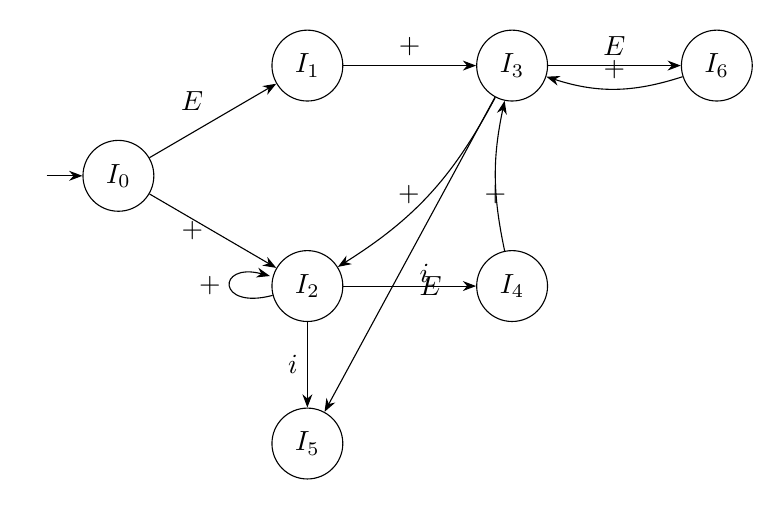
\begin{tikzpicture}[
  >=Stealth, node distance=20mm,
  every state/.style={minimum size=9mm}, initial text={}
]
  \node[state, initial] (I0) at (0,0) {$I_0$};
  \node[state] (I1) at (2.4,1.4) {$I_1$};
  \node[state] (I2) at (2.4,-1.4) {$I_2$};
  \node[state] (I3) at (5.0,1.4) {$I_3$};
  \node[state] (I4) at (5.0,-1.4) {$I_4$};
  \node[state] (I5) at (2.4,-3.4) {$I_5$};
  \node[state] (I6) at (7.6,1.4) {$I_6$};

  \path[->]
    (I0) edge node[above left] {$E$} (I1)
    (I0) edge node[left] {$+$} (I2)
    (I1) edge node[above] {$+$} (I3)
    (I2) edge node[right] {$E$} (I4)
    (I2) edge[loop left] node[left] {$+$} (I2)
    (I2) edge node[left] {$i$} (I5)
    (I3) edge node[above] {$E$} (I6)
    (I3) edge[bend left=15] node[left] {$+$} (I2)
    (I3) edge node[below right=0pt] {$i$} (I5)
    (I4) edge[bend left=12] node[below] {$+$} (I3)
    (I6) edge[bend left=18] node[above] {$+$} (I3);
\end{tikzpicture}
\end{center}

\subsection*{6.3 冲突分析}

先求 FOLLOW 集。$E$ 是开始符号（经 $S'\gto E$），故 $\#\in FOLLOW(E)$；又由 $E\gto E+E$ 知 $+\in FOLLOW(E)$。所以
\[
FOLLOW(E)=\{+,\ \#\}.
\]

\textbf{存在两个移进-归约冲突，且 SLR(1) 也无法消解：}

\begin{itemize}[leftmargin=2.2em]
  \item \ans{状态 $I_4$}：含归约项目 $E\gto +E\cdot$ 与移进项目 $E\gto E\cdot +E$。归约要求的输入是 $FOLLOW(E)=\{+,\#\}$，其中 $+$ 同时又是移进符号，因此在 $+$ 上\textbf{移进-归约冲突}。
  \item \ans{状态 $I_6$}：含归约项目 $E\gto E+E\cdot$ 与移进项目 $E\gto E\cdot +E$。同理在 $+$ 上\textbf{移进-归约冲突}。
\end{itemize}

因为归约用的 $FOLLOW(E)$ 里含有移进符号 $+$，SLR(1) 不能区分，所以这是真正的二义文法引起的冲突（与第五题“$E\gto E+E$ 无结合性”一致）。

\subsection*{6.4 任意消除其中一个}

按题目要求消除一个即可。取\textbf{状态 $I_6$} 的冲突，规定 $+$ \textbf{左结合}：

\[
\boxed{\text{在 } I_6 \text{ 遇到输入 } + \text{ 时，选择按 } E\gto E+E \text{ 归约（reduce），不移进。}}
\]

理由：左结合意味着先把左边已凑齐的 $E+E$ 规约掉，再处理后续的 $+$。这样 $I_6$ 在 $+$ 上只保留归约动作，移进-归约冲突被消除。（若要消 $I_4$，同理可令一元 $+$ 优先级更高、在 $+$ 上选择归约 $E\gto +E$。）


\section*{七、语义分析（15 分）}
\chapters{Slides：\kw{第九章2026.pdf}、\kw{第十章2026.pdf}；笔记：第 9 章“符号表、声明语义分析、函数声明、综合属性与继承属性”，第 10 章“三地址码、四元式、短路求值、数组访问、函数调用”。}

程序段：
\begin{lstlisting}
int a[2, 3];
void f(int b(), int k){
    if(k > 0 && k < 3) a[k-1,k] = b(k, 1)
    else print 0;
}
\end{lstlisting}

\subsection*{7.1 对 \kw{f} 函数声明行做语义分析（符号表）}

涉及两张表：全局表，以及 \kw{f} 的局部/参数表。

\textbf{全局符号表}（\kw{int a[2,3];} 与 \kw{f} 同层）：

\begin{center}
\begin{tabular}{c|c|L{0.42\textwidth}|c|c}
name & kind & type / 说明 & width & offset\\
\hline
\kw{a} & array & 元素 \kw{int}，\kw{dims=[2,3]}，行优先 & $2{\times}3{\times}4=24$ & 0\\
\kw{f} & function & \kw{returnType=void}，\kw{paramNum=2}，\kw{paramList=[b,k]}，指向 \kw{f} 的局部表 & --- & 24\\
\end{tabular}
\end{center}

\kw{a} 的宽度：二维数组 \kw{int[2,3]}，元素 \kw{int} 占 4，共 $2{\times}3=6$ 个，故 $width=24$；\kw{f} 紧随其后，偏移从 24 起。

\textbf{分析 \kw{void f(int b(), int k)} 的步骤：}
\begin{enumerate}[label=(\arabic*)]
  \item \textbf{登记函数名}：在全局表查 \kw{f} 是否重定义（无同名，通过），登记 \kw{f}，\kw，\kw{returnType=void}。
  \item \textbf{新建 \kw{f} 的局部表}：\kw{newtab()}，\kw{parent} 指向全局表，层次加深一层；全局表中 \kw{f} 的 \kw{entry} 指向该子表。
  \item \textbf{逐个登记形参}（从左到右）：
    \begin{itemize}[leftmargin=1.6em]
      \item \kw{int b()}：\kw{b} 是\textbf{函数型形参}（参数本身是函数，返回 \kw{int}、无参数）。它不是普通变量，运行时要携带\textbf{入口地址}和\textbf{环境信息}（访问链/静态链），故 \kw。
      \item \kw{int k}：普通整型形参，\kw，\kw{type=int}，\kw{width=4}。
    \end{itemize}
  \item \textbf{回填函数信息}：更新 \kw{f} 的 \kw{paramNum=2}、\kw{paramList=[b,k]}、参数区总宽度。
\end{enumerate}

\textbf{\kw{f} 的局部/参数符号表}：

\begin{center}
\begin{tabular}{c|c|L{0.40\textwidth}|c|c}
name & kind & type / 说明 & width & offset\\
\hline
\kw{b} & funcParam & 函数形参，\kw{returnType=int}，无参数；存“入口地址 + 环境” & 按机器（如 8） & 0\\
\kw{k} & param & \kw{int} 形参 & 4 & 接 \kw{b} 之后\\
\end{tabular}
\end{center}

\textbf{关键考点}：\kw{b} 是“函数当参数”，不能只当成一个 \kw{int}。普通变量只占一个数据宽度，而函数形参要记\textbf{入口地址}（去哪执行）和\textbf{环境信息}（按什么作用域取非局部名）。

\textbf{自然语言版}：声明了一个全局函数 \kw{f}，返回 \kw{void}，两个参数；第一个参数 \kw{b} 是返回 \kw{int} 的函数（作为参数传入，运行时带入口地址和环境），第二个参数 \kw{k} 是 \kw{int}。在全局表登记 \kw{f} 并建立其作用域，把 \kw{b}、\kw{k} 登记到参数表，最后回填参数个数、参数类型表和返回类型。


\subsection*{7.2 对 if 语句写三地址码 / 四元式}

控制结构：\kw{k>0 \&\& k<3} 用短路（\kw{k>0} 假就直接跳 else）；then 分支是数组赋值 \kw{a[k-1,k]=b(k,1)}，结束后跳过 else。

\textbf{带标签三地址码}（最直观）：

\begin{lstlisting}
        if k > 0 goto L1     // k>0 真才判断 k<3（&& 短路）
        goto Lelse           // k>0 假，整体假
L1:     if k < 3 goto Lthen
        goto Lelse
Lthen:  t1 = k - 1           // 下标 k-1
        t2 = t1 * 3          // 行优先 (i*n+j)，n=3，i=k-1，j=k
        t3 = t2 + k
        param k              // b(k,1)：从左到右传参
        param 1
        t4 = call b, 2       // 调用 b，2 个参数，返回值入 t4
        a[t3] = t4           // 写回数组元素 a[k-1,k]
        goto Lend            // then 结束，跳过 else
Lelse:  print 0
Lend:
\end{lstlisting}

要点：
\begin{itemize}[leftmargin=2.2em]
  \item \textbf{\kw{\&\&} 短路}：\kw{k>0} 真链进入 \kw{k<3} 判断，假链直接到 \kw{Lelse}；两条件都真才进 \kw{Lthen}。
  \item \textbf{数组下标 \kw{a[k-1,k]}}：声明 \kw{a[2,3]}，行优先偏移 $(i\cdot n+j)$，这里 $i=k-1$、$j=k$、$n=3$，算出的是\textbf{元素编号}。若要字节地址，再乘宽度 4：\kw{t3 = t3 * 4}，写成 \kw{M[base(a)+t3] = t4}。
  \item \textbf{函数调用 \kw{b(k,1)}}：先 \kw{param} 传参（无约定时从左到右），再 \kw{call b, 2}；\kw{b} 是函数型形参，运行时按符号表里记的入口地址和环境调用。
\end{itemize}

\textbf{四元式}（$(op,arg1,arg2,result)$，跳转的 result 为目标四元式编号，自 100 起）：

\begin{center}
\begin{tabular}{c|c|c|c|c}
编号 & op & arg1 & arg2 & result\\
\hline
100 & $j>$ & \kw{k} & \kw{0} & 102\\
101 & $j$ & \_ & \_ & 112\\
102 & $j<$ & \kw{k} & \kw{3} & 104\\
103 & $j$ & \_ & \_ & 112\\
104 & $-$ & \kw{k} & \kw{1} & \kw{t1}\\
105 & $*$ & \kw{t1} & \kw{3} & \kw{t2}\\
106 & $+$ & \kw{t2} & \kw{k} & \kw{t3}\\
107 & \kw{param} & \kw{k} & \_ & \_\\
108 & \kw{param} & \kw{1} & \_ & \_\\
109 & \kw{call} & \kw{b} & \kw{2} & \kw{t4}\\
110 & $[]{=}$ & \kw{t3} & \kw{t4} & \kw{a}\\
111 & $j$ & \_ & \_ & 113\\
112 & \kw{print} & \kw{0} & \_ & \_\\
113 & \dots & & & （后续语句）\\
\end{tabular}
\end{center}

说明：$j>$/$j<$ 表示“条件成立跳转到 result 指定编号”，$j$ 是无条件跳转，$[]{=}$ 表示数组元素赋值 \kw{a[t3]=t4}。100/102 的真出口经反填指向各自的下一段；101/103 的假出口反填到 else 入口 112。第 110 条之后用 111 无条件跳过 else（跳到 113）。具体标号衔接可按课件标号方式微调。

\textbf{说明：}本题与笔记“第 9 章·例题：2024 语义分析”一致，可对照复习。

\section*{八、运行时存储空间组织（10 分）}
\chapters{Slides：\kw{第十一章2026.pdf}；笔记：第 11 章“活动树、栈帧/活动记录、控制链与访问链、参数传递、栈快照通用步骤”。}

\subsection*{8.1 题面修正}

回忆版程序段有笔误，按要求统一并修正成\textbf{语义自洽}的版本（修正点：\kw{raw}$\to$\kw{row}；\kw{soo} 作为“函数型形参”，被调用时统一带一个实参 \kw{soo(x)}；\kw{bar} 递归时把当前的 \kw{soo} 继续往下传）：

\begin{lstlisting}
int foo(int y){
    int z;
    void bar(int x, int soo()){
        if(x > 3) bar(x/3, soo);   // 把函数 soo 继续往下传
        else z = soo(x);            // 调用函数型形参 soo
        print z;
    }
    int row(int x){
        y = x + 5;
        return y;                   // <== 求执行到这里时的栈快照
    }
    bar(y, row);                    // 把函数 row 作为参数传给 bar
}
foo(6);
\end{lstlisting}

\textbf{词法嵌套关系}：\kw{bar} 和 \kw{row} 都直接声明在 \kw{foo} 内，所以两者的\textbf{访问链}都指向 \kw{foo} 的活动记录。

\subsection*{8.2 调用链推演}

\begin{enumerate}[label=(\arabic*)]
  \item \kw{foo(6)}：\kw{y=6}。执行 \kw{bar(y, row)}，即 \kw{bar(6, row)}，把函数 \kw{row}（连同它的环境 \kw{foo}）作为参数 \kw{soo} 传入。
  \item \kw{bar(6, row)}：\kw{x=6>3} 成立，递归 \kw{bar(6/3, soo)}，即 \kw{bar(2, row)}，\kw{soo} 继续是 \kw{row}。
  \item \kw{bar(2, row)}：\kw{x=2>3} 不成立，走 else，执行 \kw{z = soo(x)}，即 \kw{z = row(2)}。
  \item \kw{row(2)}：\kw{y = 2 + 5 = 7}，执行到 \ans{\kw{return y;}}。此刻栈顶是 \kw{row} 的活动记录。
\end{enumerate}

因此运行到 \kw{return y;} 时，栈上由底到顶依次有 4 个活动记录：
\[
\kw{foo(6)}\ \to\ \kw{bar(6,row)}\ \to\ \kw{bar(2,row)}\ \to\ \kw{row(2)}.
\]

\textbf{此刻的值}：\kw{y} 已被 \kw{row} 改成 \kw{7}；\kw{z} 还未赋值（\kw{z=row(2)} 的右边正在求值，赋值尚未完成），故 \kw{z} 仍为未定义。

\subsection*{8.3 栈快照}

按题图字段顺序（形参 / 访问链 / 控制链 / 返回地址 / 变量）自底向上填写。\kw{y}、\kw{z} 是 \kw{foo} 的数据，登记在 \kw{foo} 的活动记录里；函数型实参 \kw{soo} 携带一对值“代码入口 + 环境”，环境即声明它的 \kw{foo} 活动记录。用记号 \kw{AR(p)} 表示过程 \kw{p} 本次活动的活动记录基址。

\begin{center}
\begin{longtable}{c|l|l}
活动记录 & 单元（字段） & 内容 / 说明\\
\hline
\multirow{3}{*}{\kw{foo(6)}}
 & 形参 \kw{y} & \kw{7}（初值 6，已被 \kw{row} 改写为 $2+5$）\\
 & 控制链 & 指向调用者（主程序/\kw{\#}）\\
 & 局部变量 \kw{z} & 未定义（\kw{z=row(2)} 尚未赋值）\\
\hline
\multirow{5}{*}{\shortstack[l]{\kw{bar(6,row)}\\第 1 次}}
 & 形参 \kw{x} & \kw{6}\\
 & 形参 \kw{soo} & (\kw{row@入口}, \kw{AR(foo)})，即 \kw{row} 的代码入口 + 环境 \kw{foo}\\
 & 访问链 & 指向 \kw{AR(foo)}（\kw{bar} 声明在 \kw{foo} 内）\\
 & 控制链 & 指向 \kw{AR(foo)}（调用者是 \kw{foo}）\\
 & 返回地址 & \kw{foo} 中 \kw{bar(y,row)} 之后\\
\hline
\multirow{5}{*}{\shortstack[l]{\kw{bar(2,row)}\\第 2 次（递归）}}
 & 形参 \kw{x} & \kw{2}（$=6/3$）\\
 & 形参 \kw{soo} & (\kw{row@入口}, \kw{AR(foo)})，由上一层 \kw{bar} 原样传下\\
 & 访问链 & 指向 \kw{AR(foo)}（仍按声明环境，\textbf{不是}调用者）\\
 & 控制链 & 指向第 1 次 \kw{bar} 的活动记录（调用者）\\
 & 返回地址 & \kw{bar} 中 \kw{if} 的 then 分支 \kw{bar(x/3,soo)} 之后\\
\hline
\multirow{4}{*}{\kw{row(2)}}
 & 形参 \kw{x} & \kw{2}\\
 & 访问链 & 指向 \kw{AR(foo)}（\kw{row} 声明在 \kw{foo} 内；由 \kw{soo} 携带的环境得到）\\
 & 控制链 & 指向第 2 次 \kw{bar} 的活动记录（调用者）\\
 & 返回地址 & \kw{bar} 中 \kw{z=soo(x)} 的赋值处\\
\hline
\end{longtable}
\end{center}

\textbf{两条链的要点}（本题最易错处）：
\begin{itemize}[leftmargin=2.2em]
  \item \textbf{访问链}按\textbf{词法嵌套}（声明位置）设置：\kw{bar}、\kw{row} 都声明在 \kw{foo} 内，所以三个活动记录的访问链\textbf{都指向 \kw{foo}}，与“谁调用谁”无关。\kw{row} 被当作 \kw{soo} 间接调用，它的访问链也来自传入的环境 \kw{AR(foo)}。
  \item \textbf{控制链}按\textbf{调用顺序}设置：\kw{row} 的控制链指向第 2 次 \kw{bar}，第 2 次 \kw{bar} 的控制链指向第 1 次 \kw{bar}，第 1 次 \kw{bar} 的控制链指向 \kw{foo}。
  \item \textbf{函数型形参 \kw{soo}}：不是普通整数，存的是一对“代码入口 + 环境”。正因为带了环境 \kw{AR(foo)}，\kw{row} 里的非局部名 \kw{y} 才能正确地找到 \kw{foo} 的 \kw{y} 并改成 7。
\end{itemize}

\textbf{说明：}回忆版未给出具体地址数值与帧指针标法，本表用符号 \kw{AR(p)} 表达链的指向关系；若老师要求填具体地址，可仿照 \kw{exam\_17} 第 7 题，从高地址往低地址给每个单元编号即可，链值改成对应单元地址。


\end{document}
